% Options for packages loaded elsewhere
\PassOptionsToPackage{unicode}{hyperref}
\PassOptionsToPackage{hyphens}{url}
%
\documentclass[
  ignorenonframetext,
]{beamer}
\usepackage{pgfpages}
\setbeamertemplate{caption}[numbered]
\setbeamertemplate{caption label separator}{: }
\setbeamercolor{caption name}{fg=normal text.fg}
\beamertemplatenavigationsymbolsempty
% Prevent slide breaks in the middle of a paragraph
\widowpenalties 1 10000
\raggedbottom
\setbeamertemplate{part page}{
  \centering
  \begin{beamercolorbox}[sep=16pt,center]{part title}
    \usebeamerfont{part title}\insertpart\par
  \end{beamercolorbox}
}
\setbeamertemplate{section page}{
  \centering
  \begin{beamercolorbox}[sep=12pt,center]{part title}
    \usebeamerfont{section title}\insertsection\par
  \end{beamercolorbox}
}
\setbeamertemplate{subsection page}{
  \centering
  \begin{beamercolorbox}[sep=8pt,center]{part title}
    \usebeamerfont{subsection title}\insertsubsection\par
  \end{beamercolorbox}
}
\AtBeginPart{
  \frame{\partpage}
}
\AtBeginSection{
  \ifbibliography
  \else
    \frame{\sectionpage}
  \fi
}
\AtBeginSubsection{
  \frame{\subsectionpage}
}
\usepackage{amsmath,amssymb}
\usepackage{lmodern}
\usepackage{ifxetex,ifluatex}
\ifnum 0\ifxetex 1\fi\ifluatex 1\fi=0 % if pdftex
  \usepackage[T1]{fontenc}
  \usepackage[utf8]{inputenc}
  \usepackage{textcomp} % provide euro and other symbols
\else % if luatex or xetex
  \usepackage{unicode-math}
  \defaultfontfeatures{Scale=MatchLowercase}
  \defaultfontfeatures[\rmfamily]{Ligatures=TeX,Scale=1}
  \setmainfont[BoldFont = SF Pro Rounded Semibold]{SF Pro Rounded}
  \setmathfont[]{STIX Two Math}
\fi
\usefonttheme{serif} % use mainfont rather than sansfont for slide text
% Use upquote if available, for straight quotes in verbatim environments
\IfFileExists{upquote.sty}{\usepackage{upquote}}{}
\IfFileExists{microtype.sty}{% use microtype if available
  \usepackage[]{microtype}
  \UseMicrotypeSet[protrusion]{basicmath} % disable protrusion for tt fonts
}{}
\makeatletter
\@ifundefined{KOMAClassName}{% if non-KOMA class
  \IfFileExists{parskip.sty}{%
    \usepackage{parskip}
  }{% else
    \setlength{\parindent}{0pt}
    \setlength{\parskip}{6pt plus 2pt minus 1pt}}
}{% if KOMA class
  \KOMAoptions{parskip=half}}
\makeatother
\usepackage{xcolor}
\IfFileExists{xurl.sty}{\usepackage{xurl}}{} % add URL line breaks if available
\IfFileExists{bookmark.sty}{\usepackage{bookmark}}{\usepackage{hyperref}}
\hypersetup{
  pdftitle={305 Lecture 4.6 - Rules for And},
  pdfauthor={Brian Weatherson},
  hidelinks,
  pdfcreator={LaTeX via pandoc}}
\urlstyle{same} % disable monospaced font for URLs
\newif\ifbibliography
\usepackage{graphicx}
\makeatletter
\def\maxwidth{\ifdim\Gin@nat@width>\linewidth\linewidth\else\Gin@nat@width\fi}
\def\maxheight{\ifdim\Gin@nat@height>\textheight\textheight\else\Gin@nat@height\fi}
\makeatother
% Scale images if necessary, so that they will not overflow the page
% margins by default, and it is still possible to overwrite the defaults
% using explicit options in \includegraphics[width, height, ...]{}
\setkeys{Gin}{width=\maxwidth,height=\maxheight,keepaspectratio}
% Set default figure placement to htbp
\makeatletter
\def\fps@figure{htbp}
\makeatother
\setlength{\emergencystretch}{3em} % prevent overfull lines
\providecommand{\tightlist}{%
  \setlength{\itemsep}{0pt}\setlength{\parskip}{0pt}}
\setcounter{secnumdepth}{-\maxdimen} % remove section numbering
\let\Tiny=\tiny

 \setbeamertemplate{navigation symbols}{} 

% \usetheme{Madrid}
 \usetheme[numbering=none, progressbar=foot]{metropolis}
 \usecolortheme{wolverine}
 \usepackage{color}
 \usepackage{MnSymbol}
% \usepackage{movie15}

\usepackage{amssymb}% http://ctan.org/pkg/amssymb
\usepackage{pifont}% http://ctan.org/pkg/pifont
\newcommand{\cmark}{\ding{51}}%
\newcommand{\xmark}{\ding{55}}%

\DeclareSymbolFont{symbolsC}{U}{txsyc}{m}{n}
\DeclareMathSymbol{\boxright}{\mathrel}{symbolsC}{128}
\DeclareMathAlphabet{\mathpzc}{OT1}{pzc}{m}{it}

 \usepackage{tikz-qtree}
% \usepackage{markdown}
%\RequirePackage{bussproofs}
\RequirePackage[tableaux]{prooftrees}
\usetikzlibrary{arrows.meta}
 \forestset{line numbering, close with = x}
% Allow for easy commas inside trees
\renewcommand{\,}{\text{, }}


\usepackage{tabulary}

\usepackage{open-logic-config}

\setlength{\parskip}{1ex plus 0.5ex minus 0.2ex}

\AtBeginSection[]
{
\begin{frame}
	\Huge{\color{darkblue} \insertsection}
\end{frame}
}

\renewenvironment*{quote}	
	{\list{}{\rightmargin   \leftmargin} \item } 	
	{\endlist }

\definecolor{darkgreen}{rgb}{0,0.7,0}
\definecolor{darkblue}{rgb}{0,0,0.8}

\newcommand{\starttab}{\begin{center}
\vspace{6pt}
\begin{tabular}}

\newcommand{\stoptab}{\end{tabular}
\vspace{6pt}
\end{center}
\noindent}


\newcommand{\sif}{\rightarrow}
\newcommand{\siff}{\leftrightarrow}
\newcommand{\EF}{\end{frame}}


\newcommand{\TreeStart}[1]{
%\end{frame}
\begin{frame}
\begin{center}
\begin{tikzpicture}[scale=#1]
\tikzset{every tree node/.style={align=center,anchor=north}}
%\Tree
}

\newcommand{\TreeEnd}{
\end{tikzpicture}
%\end{center}
}

\newcommand{\DisplayArg}[2]{
\begin{enumerate}
{#1}
\end{enumerate}
\vspace{-6pt}
\hrulefill

%\hspace{14pt} #2
%{\addtolength{\leftskip}{14pt} #2}
\begin{quote}
{\normalfont #2}
\end{quote}
\vspace{12pt}
}

\newenvironment{ProofTree}[1][1]{
\begin{center}
\begin{tikzpicture}[scale=#1]
\tikzset{every tree node/.style={align=center,anchor=south}}
}
{
\end{tikzpicture}
\end{center}
}

\newcommand{\TreeFrame}[2]{
\begin{columns}[c]
\column{0.5\textwidth}
\begin{center}
\begin{prooftree}{}
#1
\end{prooftree}
\end{center}
\column{0.45\textwidth}
%\begin{markdown}
#2
%\end{markdown}
\end{columns}
}

\newcommand{\ScaledTreeFrame}[3]{
\begin{columns}[c]
\column{0.5\textwidth}
\begin{center}
\scalebox{#1}{
\begin{prooftree}{}
#2
\end{prooftree}
}
\end{center}
\column{0.45\textwidth}
%\begin{markdown}
#3
%\end{markdown}
\end{columns}
}

\usepackage[bb=boondox]{mathalfa}
\DeclareMathAlphabet{\mathbx}{U}{BOONDOX-ds}{m}{n}
\SetMathAlphabet{\mathbx}{bold}{U}{BOONDOX-ds}{b}{n}
\DeclareMathAlphabet{\mathbbx} {U}{BOONDOX-ds}{b}{n}


\newenvironment{oltableau}{\center\tableau{}} %wff format={anchor = base west}}}
       {\endtableau\endcenter}
       
\newcommand{\formula}[1]{$#1$}

\usepackage{tabulary}
\usepackage{booktabs}

\def\begincols{\begin{columns}}
\def\begincol{\begin{column}}
\def\endcol{\end{column}}
\def\endcols{\end{columns}}

\usepackage[italic]{mathastext}
\usepackage{nicefrac}

\definecolor{mygreen}{RGB}{0, 100, 0}
\definecolor{mypink2}{RGB}{219, 48, 122}
\definecolor{dodgerblue}{RGB}{30,144,255}

%\def\True{\textcolor{dodgerblue}{\text{T}}}
%\def\False{\textcolor{red}{\text{F}}}

\def\True{\mathbb{T}}
\def\False{\mathbb{F}}

% This is because arguments didn't have enough space after them
\usepackage{etoolbox}
\AfterEndEnvironment{description}{\vspace{9pt}}
\AfterEndEnvironment{oltableau}{\vspace{9pt}}
\BeforeBeginEnvironment{oltableau}{\vspace{9pt}}
\AfterEndEnvironment{center}{\vspace{12pt}}
\BeforeBeginEnvironment{tabular}{\vspace{9pt}}

\setlength\heavyrulewidth{0pt}
\setlength\lightrulewidth{0pt}

%\def\toprule{}
%\def\bottomrule{}
%\def\midrule{}

\setbeamertemplate{caption}{\raggedright\insertcaption}

\ifluatex
  \usepackage{selnolig}  % disable illegal ligatures
\fi

\title{305 Lecture 4.6 - Rules for And}
\author{Brian Weatherson}
\date{}

\begin{document}
\frame{\titlepage}

\begin{frame}{Plan}
\protect\hypertarget{plan}{}
This lecture introduces the two rules for \(\wedge\).
\end{frame}

\begin{frame}{Associated Reading}
\protect\hypertarget{associated-reading}{}
forall x, section 16.3.
\end{frame}

\begin{frame}{Reasoning from And sentences}
\protect\hypertarget{reasoning-from-and-sentences}{}
If you know that it snowed in Detroit and it snowed in Ann Arbor, there
are two natural things you can infer. \pause

\begin{enumerate}
\tightlist
\item
  It snowed in Detroit. \pause
\item
  It snowed in Ann Arbor
\end{enumerate}
\end{frame}

\begin{frame}{And-Elimination}
\protect\hypertarget{and-elimination}{}
\begin{itemize}
\tightlist
\item
  And-elimination, or \(\wedge\)E, is the formal version of the idea
  behind the last slide.
\item
  It is in fact a pair of rules.
\item
  The first says that from a conjunction you can infer the first
  conjunct.
\item
  The second says that from a conjunction you can infer the second
  conjunct.
\end{itemize}
\end{frame}

\begin{frame}{And-Elimination the first}
\protect\hypertarget{and-elimination-the-first}{}
\begin{figure}
\centering
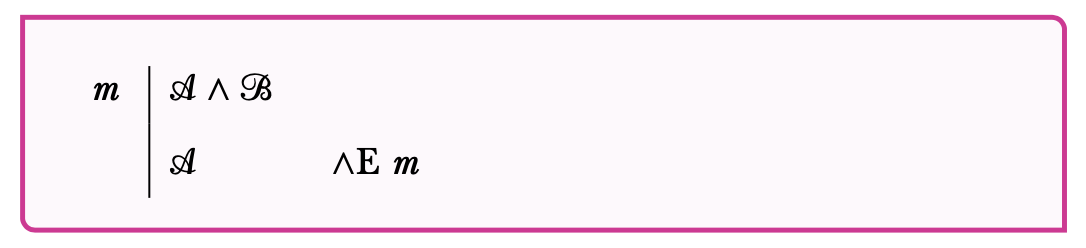
\includegraphics{4_6a.png}
\caption{First Form of And-Elimination}
\end{figure}
\end{frame}

\begin{frame}{And-Elimination the second}
\protect\hypertarget{and-elimination-the-second}{}
\begin{figure}
\centering
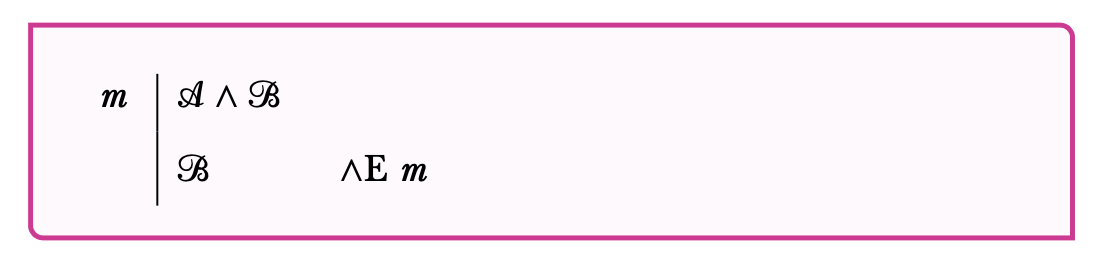
\includegraphics{4_6b.png}
\caption{Second Form of And-Elimination}
\end{figure}
\end{frame}

\begin{frame}{A Key Constraint}
\protect\hypertarget{a-key-constraint}{}
\begin{itemize}
\tightlist
\item
  Just like with trees, these rules only apply to whole lines.
\item
  So you can only apply \(\wedge\)E to a line if it has \(\wedge\) as
  its \textbf{main connective}.
\item
  Remember, \(\wedge\) is the main connective if there is a well formed
  sentence either side of it.
\end{itemize}
\end{frame}

\begin{frame}{Reasoning to an And sentence}
\protect\hypertarget{reasoning-to-an-and-sentence}{}
How might we prove a conjunctive sentence, say that it snowed in Detroit
and it snowed in Ann Arbor? \pause There are a lot of ways we could do
it, but the most obvious involves:

\begin{enumerate}
\tightlist
\item
  Proving that it snowed in Detroit.
\item
  Proving that it snowed in Ann Arbor.
\item
  Declaring victory.
\end{enumerate}
\end{frame}

\begin{frame}{And-Introduction}
\protect\hypertarget{and-introduction}{}
\begin{itemize}
\tightlist
\item
  And-introduction, or \(\wedge\)I, is the formal version of the idea
  behind the last slide.
\item
  It says that if you have a pair of sentences, you can infer the
  conjunction of those two sentences.
\item
  It doesn't matter which order the sentences appear in the proof.
\end{itemize}
\end{frame}

\begin{frame}{And-Introduction}
\protect\hypertarget{and-introduction-1}{}
\begin{figure}
\centering
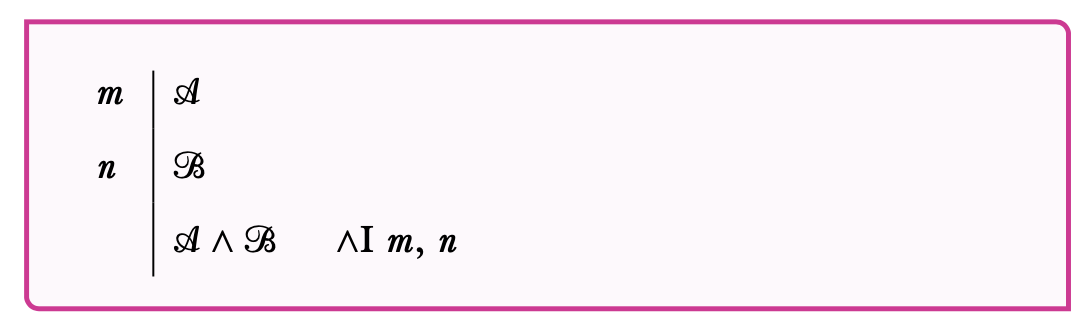
\includegraphics{4_6c.png}
\caption{And-Elimination}
\end{figure}
\end{frame}

\begin{frame}{A Proof}
\protect\hypertarget{a-proof}{}
\begin{columns}[c]
\begin{column}{0.48\textwidth}
\begin{figure}
\centering
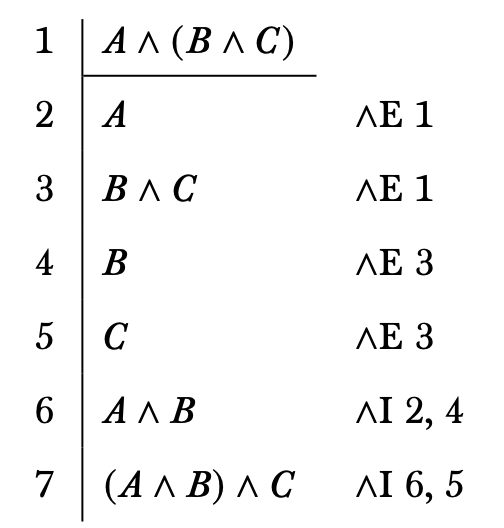
\includegraphics{4_6d.png}
\caption{Our first proof}
\end{figure}
\end{column}

\begin{column}{0.48\textwidth}
\begin{itemize}
\tightlist
\item
  This proof starts with one premise.
\item
  The next four lines consist of taking that premise apart.
\item
  And the next two consist of putting it back together, the way we want.
\end{itemize}
\end{column}
\end{columns}
\end{frame}

\begin{frame}{Where We're At}
\protect\hypertarget{where-were-at}{}
\begin{itemize}
\tightlist
\item
  What I care about for now is that you understand how to read this
  proof.
\item
  Figuring out how to construct a proof like this is harder, and that's
  something we'll spend a lot of time on next week.
\item
  Natural deduction proofs should be much easier to read than to write.
\end{itemize}
\end{frame}

\begin{frame}{For Next Time}
\protect\hypertarget{for-next-time}{}
\begin{itemize}
\tightlist
\item
  We will look at 16.4, on the rules for `if'.
\end{itemize}
\end{frame}

\end{document}
